% Este arquivo tex vai ser incluído no arquivo tex principal, não pe preciso
% declarar nenhum cabeçalho

\section{Bem-vindo a um mundo novo!}

Olá, bixo! Seja bem-vindo! Agora que você está na faculdade, pode ser que aprenda que aquele estereótipo de nerd
da escola não lhe garante boas notas, e que o lugar onde você mais vai aprender não
é a sala de aula. É verdade, calouro, a faculdade é diferente, e quase tudo
dependerá de você, desde quais matérias quer cursar até quando vai estudar para
as provas. Portanto, leia isto com atenção.

Os professores, salvo raras exceções, dificilmente saberão seu nome ou quem é você; provavelmente, eles só verão
no final do semestre se o RA 137654  passou ou não passou. Mas não se sinta
desamparado, afinal, você também vai logo esquecer a matéria deles! O quanto você
estuda não é diretamente proporcional à sua nota, portanto aprenda a estudar
melhor. Atividades em grupo, resolução de exercícios e monitorias são boas pedidas.

Mas a Universidade não se resume a estudo. Você vai conhecer muita gente nova e
descobrir que a vida acadêmica vai muito além.
Cada graduando tem uma cultura própria, e tem gente do
Brasil inteiro na Unicamp, então não se surpreenda se te chamarem de
pessoa, piá, meu, mano, jovem, moleque, guri, moço, rapaz,
brou. Essas pessoas são bem legais quando você se acostuma com essa
diversidade.

O campus é essa doideira toda mesmo. Você pode estar andando e
cruzar com alguém tocando gaita de fole, alguém parecendo uma
estátua em plena praça, ou então um grupo na grama lendo a Bíblia, treinando
Wushu ou Taijiquan. Não se sinta sozinho, afinal todos seus colegas estão assim
também e depois de um mês você estará adorando isso e perceberá porque todos
dizem que a época de faculdade é a melhor da vida.

Este manual foi organizado pelo CACo (Centro Acadêmico da Computação -- o seu
CA), para ajudá-lo nesse começo de vida universitária! Onde comer? Onde estudar?
Onde morar? Tudo isso são dúvidas comuns, que aqui tentamos ajudar a resolver.
Não há respostas prontas, cada um tem suas preferências, mas a gente dá uma mão.

O que é CA? E Atlética? E DCE? E Bandejão? E Moradia? E essas siglas e códigos
malucos? Como eu faço para pegar uma bolsa? A gente também tenta responder a todas
essas perguntas. E também damos algumas dicas de onde comprar coisas, onde se
divertir e alguns telefones úteis!

Parabéns pela aprovação! Seja bem-vindo e aproveite a vida acadêmica!

\begin{figure}[hb!]
    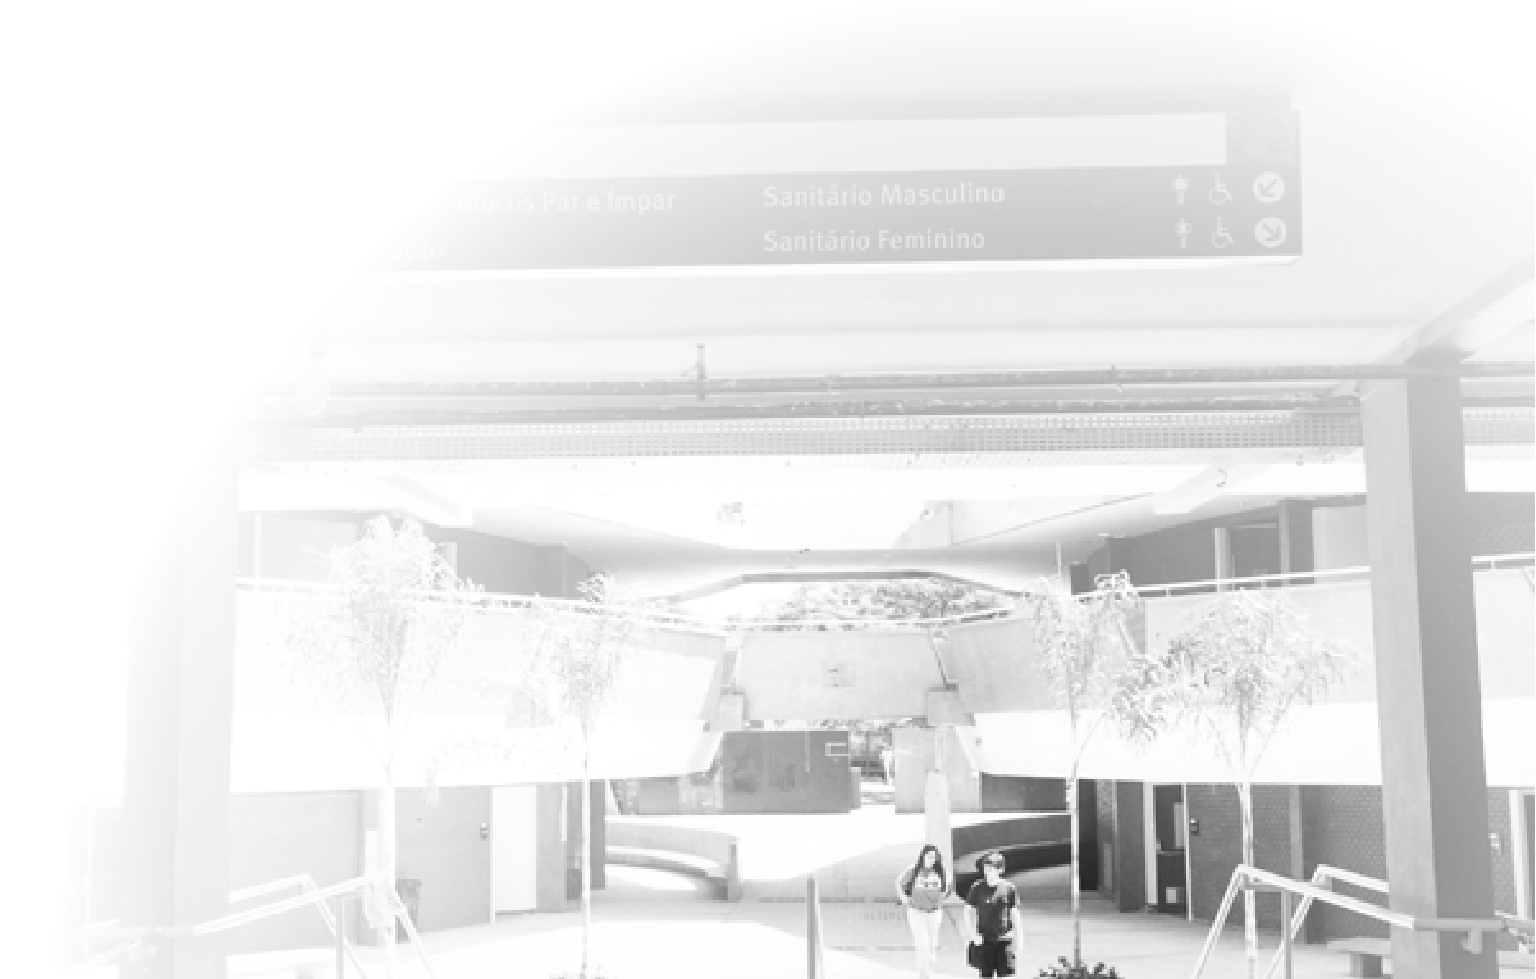
\includegraphics[scale=0.68, keepaspectratio=true]{img/imgs/1-boas_vindas/-007.jpg}
\end{figure}


